\documentclass[conference]{IEEEtran}
\IEEEoverridecommandlockouts
\usepackage{cite}
\usepackage{amsmath,amssymb,amsfonts}
\usepackage{graphicx}
\usepackage{textcomp}
\usepackage{xcolor}
\usepackage{booktabs}
\usepackage{array}
\usepackage{url}
\usepackage{tikz}
\usetikzlibrary{shapes.geometric,arrows.meta,positioning}
\tikzset{
  stage/.style  = {draw, fill=green!6, rounded corners=2pt,
                   font=\small, minimum width=3.3cm,
                   minimum height=0.62cm, align=center},
  dec/.style    = {diamond, draw, fill=blue!5,
                   font=\small, minimum width=2.4cm,
                   minimum height=0.8cm, aspect=1.8, align=center},
  arr/.style    = {-Stealth, thick},
}
\begin{document}
\title{StudyMate: Curriculum-Grounded Retrieval,\\
Abstention, and Grounding Audits\\
for Educational Question Answering}
\author{
\IEEEauthorblockN{Dr.\ B Swathi}
\IEEEauthorblockA{Dept.\ of CSE (Data Science)\\
New Horizon College of Engineering\\
Bengaluru, India\\
basawarajus@newhorizonindia.edu}
\and
\IEEEauthorblockN{Monish V}
\IEEEauthorblockA{Dept.\ of CSE (Data Science)\\
New Horizon College of Engineering\\
Bengaluru, India\\
1nh23cd092@newhorizonindia.edu}
\and
\IEEEauthorblockN{Manprit}
\IEEEauthorblockA{Dept.\ of CSE (Data Science)\\
New Horizon College of Engineering\\
Bengaluru, India\\
1nh23cd087@newhorizonindia.edu}
\and
\IEEEauthorblockN{Sinchana R M}
\IEEEauthorblockA{Dept.\ of CSE (Data Science)\\
New Horizon College of Engineering\\
Bengaluru, India\\
1nh23cd165@newhorizonindia.edu}
\and
\IEEEauthorblockN{Sushmitha Yadwad}
\IEEEauthorblockA{Dept.\ of CSE (Data Science)\\
New Horizon College of Engineering\\
Bengaluru, India\\
1nh23cd172@newhorizonindia.edu}
}
\maketitle
% Uncomment once ICICF sends the publication-rights string.
% \IEEEpubid{\makebox[\columnwidth]{XXX-X-XXXX-XXXX-X/XX/\$XX.00~\copyright2027 IEEE \hfill} \hspace{\columnsep}\makebox[\columnwidth]{}}

\begin{abstract}
Curriculum-specific question answering requires more than fluent generation:
retrieved passages must match the syllabus, unsupported answers should be
withheld, and citations must genuinely support the generated claims. We
present \textit{StudyMate}, a retrieval-augmented teaching assistant for
Karnataka Pre-University and CBSE learners, combining board-conditioned
answer formatting, hybrid retrieval, a corrective retrieval loop, an evidence
floor and post-generation grounding audits. Evaluation uses a 174-item
curriculum benchmark: 150 answerable board-paper questions and 24
out-of-syllabus questions. Five findings characterise the implementation.
First, dense similarity can retrieve irrelevant front matter despite high
ranking scores. Second, a small corrective-retrieval grader can reject useful
evidence: in a 40-question ablation it falsely abstained on 11 items, while a
stronger grader matched the plain baseline's abstention recall at roughly 29
percent greater latency. Third, a similarity-gated evidence floor reduced
false abstentions from 8 of 40 to 2 of 40 and raised abstention precision from
7 of 15 to 7 of 9 in a separate paired run; the threshold was selected on the
same benchmark, so these are exploratory results. Fourth, an audit of 300
generated statements found 78 percent traceable to provided evidence, but only
6.5 percent citing the supporting passage. Fifth, two judges scoring 22
identical answers showed unstable faithfulness estimates, with a near-zero
correlation; persona-style consistency was also low on nine activated
examples, between 0.22 and 0.33. These findings favour measurable retrieval,
abstention and attribution safeguards over unverified claims of teaching
effectiveness. Answer correctness and learner outcomes remain unmeasured
pending expert and participant evaluation.
\end{abstract}

\begin{IEEEkeywords}
Retrieval-Augmented Generation, Corrective RAG, Educational Chatbot, Curriculum
Question Answering, Bloom's Taxonomy, Abstention, Persona-Conditioned
Generation, Benchmark, Multilingual NLP
\end{IEEEkeywords}

%------------------------------------------------
\section{Introduction}
%------------------------------------------------
Students preparing for board examinations guess which topics recur from old
papers, queue for one lecturer stretched across a hundred learners, and fall
back on a general chatbot that has never seen their syllabus. None of these
routes scales~\cite{lauber2025}. One-to-one tutoring has long motivated research
into scalable learning support, although Bloom's ``two sigma'' observation
should not be taken as a performance prediction for AI
tutors~\cite{bloom1984,vanlehn2011}. The catch is well known --- a model leaning
on pre-trained weights states things that sound right but drift from the course
material~\cite{lewis2020} --- and Retrieval-Augmented Generation (RAG) was
introduced to fix exactly that.

This paper reports what happened when we built such a system and measured it.
Five findings shape the contribution. \textbf{Retrieval can succeed by its own
metric and fail at the task}: asking for practice-paper material returned the
textbook's preface, because front matter carries the subject name more densely
than any chapter. \textbf{A corrective loop does not automatically fix it}: a
$3$B grader implementing the grade--rewrite--abstain loop of Corrective
RAG~\cite{yan2024crag} refuses $11$ of $40$ answerable questions, and a strong
grader recovers only to match the plain baseline at $29\%$ higher latency.
\textbf{The harm is repairable without a stronger grader}: the small grader
rejects every passage, starving the generator into answering from its weights.
\textbf{A judged score describes its judge}: two judges scoring identical
answers do not agree ($r = -0.074$ on faithfulness, $\kappa = 0.182$ on style).
\textbf{Persona conditioning is bounded by the encoder}: the pipeline works for
an English-caption lecture but never fires for a Hindi-caption one against an
English corpus.

Our contributions are: (i) a $174$-item curriculum QA benchmark from real board
papers with an out-of-syllabus split; (ii) an ablation of whether corrective
retrieval earns its cost, reported as a negative result with a diagnosis and a
cheap repair; (iii) board-conditioned generation following a named board's
mark-allocation convention; (iv) a grounding audit separating invention,
misattribution and dangling citations; and (v) a two-judge evaluation showing
judged faithfulness is not stable across judges.

%------------------------------------------------
\section{Related Work}
%------------------------------------------------
RAG chatbots for education are established. Lauber \textit{et
al.}~\cite{lauber2025} align chatbot roles to pedagogy on a single German course
without an acceptance study; Teixeira \textit{et al.}~\cite{teixeira2025}
benchmark vector stores and embedding models but report no running prototype;
Neumann \textit{et al.}~\cite{neumann2025} field MoodleBot for a German database
course, reporting $88\%$ accuracy and TAM scores over $47$ participants, an
instrument we have \emph{not} yet run. KG-RAG~\cite{dong2025} adds a knowledge
graph whose maintenance annual syllabus revision makes costly, so we keep the
knowledge layer as re-indexable text; URAG~\cite{nguyen2025} routes easy queries
to keyword matching, informing our dispatcher; RAG-X~\cite{he2025} reports a
$30.3\%$ UX gain over $62$ students but is Chinese-only;
ARIA~\cite{luo2026} parses multimodal material at $97.5\%$ accuracy without
addressing board answer structure. L\'opez-Ostenero \textit{et
al.}~\cite{gielis2025} use Telegram without RAG, Koutsiaki \textit{et
al.}~\cite{koutsiaki2025} show sentence-preserving chunk boundaries beat fixed
windows, which we adopt, and Es \textit{et al.}~\cite{es2025} introduce RAGAS;
surveys~\cite{kuhail2023,wollny2021} find most systems single-purpose and rarely
multilingual.

Our corrective layer follows Yan \textit{et al.}~\cite{yan2024crag}; we claim
not the mechanism but the \emph{negative ablation}. BM25~\cite{robertson2009}
and reciprocal rank fusion~\cite{cormack2009} are standard, and checking output
against evidence is established --- SelfCheckGPT~\cite{manakul2023} by sampling,
ALCE~\cite{gao2023} by citation support --- but our evidence is fixed by
retrieval, so entailment is reserved for claims a free lexical pass flags.
Persona-conditioned agents predate RAG~\cite{liu2024persona,liu2025pace} and
embodied teachers~\cite{zhao2024} share the intuition; all personalise toward
the student. We found no comparable work conditioning the tutor's delivery on a
named educator, though this does not establish absolute novelty.

%------------------------------------------------
\section{System Architecture and Implementation Status}
%------------------------------------------------
StudyMate is thirteen loosely coupled modules behind a FastAPI service, plus
four cross-cutting mechanisms: a corrective retrieval layer, a lexical arm fused
with the dense index, an evidence floor over that layer, and a post-generation
grounding audit. A request is metadata-filtered, retrieved, graded, floored,
generated under board conventions, audited, and returned with inline citations.
Table~\ref{tab:status} distinguishes implemented from partial components.

\begin{table}[htbp]
\caption{Module implementation status and evaluated technologies.}
\label{tab:status}
\centering
\scriptsize
\setlength{\tabcolsep}{3pt}
\begin{tabular}{@{}p{0.65cm} p{1.15cm} p{5.75cm}@{}}
\toprule
\textbf{Mod.} & \textbf{Status} & \textbf{Evaluated implementation} \\
\midrule
M1 & Implemented & \textbf{FAISS} flat inner-product index, metadata filters \\
M2 & Implemented & FastAPI; \textbf{no LangChain} (direct orchestration) \\
M3 & Implemented & \textbf{Raw \texttt{httpx}} webhook client \\
M4 & Implemented & TF-IDF PYQ trends (lexical, §\ref{sec:limits}) \\
M5 & Implemented & Bloom's blueprint + structural validator \\
M6 & Implemented & Planner with retrieval-grounded subtopics \\
M7 & Implemented & \textbf{SQLite}, encrypted at rest \\
M8 & Partial & Whisper STT working; gTTS \textbf{disabled by default} \\
M9 & Partial & \textbf{JSON analytics API}, key-gated; no charts \\
M10 & Implemented & AES-256-GCM at rest, HMAC-SHA256 identifiers \\
M11 & Implemented & Deterministic strategy rule (§\ref{sec:adaptive}) \\
M12 & Implemented & \textbf{Caption retrieval library} \\
M13 & Implemented & Grammar-pinned Mermaid, structural re-emission \\
CRAG & Implemented & Corrective retrieval; ablated in §\ref{sec:ablation} \\
HYB & Implemented & BM25 fused with dense index by RRF \\
FLR & Implemented & Evidence floor over corrective layer (§\ref{sec:floor}) \\
AUD & Implemented & Post-generation grounding audit (§\ref{sec:audit}) \\
\bottomrule
\end{tabular}
\end{table}

\subsection{Retrieval and Lexical Fusion}
The corpus comprises Pre-University textbooks and board papers for physics,
chemistry, mathematics and biology across both years, chunked at $500$ tokens
with $50$-token overlap and encoded with \texttt{all-MiniLM-L6-v2} into a FAISS
inner-product index of $7{,}669$ passages; clean source material matters as much
as the model~\cite{roh2021}. Every query is filtered by subject, level, board
and document type, and passages below cosine $0.30$ are discarded. Because a
$384$-dimensional embedding blurs the rare tokens carrying most of the meaning
in a science syllabus, we add a BM25 arm~\cite{robertson2009} ($k_1=1.5$,
$b=0.75$) and fuse rankings by reciprocal rank fusion~\cite{cormack2009},
$\sum_r 1/(k + \text{rank}_r)$ with $k=60$; fusing \emph{positions} avoids
making a cosine of $0.42$ commensurate with a BM25 score of $11.3$. The lexical
index is built lazily over the $7{,}669$ passages ($48{,}010$ terms, $0.8$\,s).
A lexical-only hit is given its true cosine by reconstructing its stored vector,
so the similarity floor applies to both arms.

\subsection{Corrective Layer and Evidence Floor}
\label{sec:floor}
Each surviving passage is graded on a three-point scale (fully supports /
background only / unrelated or front matter). If the best grade reaches $0.90$
the graded passages are used; otherwise the query is rewritten into textbook
vocabulary and retrieval repeated, and if nothing usable survives the system
declines. Instrumenting the loop shows the $3$B grader does not merely misrank:
it returns $0.0$ for \emph{every} retrieved passage on questions plainly in
syllabus, and a generator given almost no evidence does not abstain but falls
back on parametric memory.

We therefore add a floor. When grading leaves fewer than $n=3$ passages but
retrieval returned candidates the dense index puts plainly on topic, those are
restored, above a higher similarity bar than the one admitting a passage for
grading. Over the benchmark the top-1 cosine for an answerable question has
median $0.602$ (range $0.234$--$0.957$) against $0.306$ ($0.201$--$0.650$) out
of syllabus: the distributions overlap and no threshold divides them. Sweeping
it trades errors directly --- at $0.40$, eleven of $150$ answerable questions
fall below and seven of $24$ out-of-syllabus rise above; at the selected $0.45$,
seventeen and four; at $0.50$, twenty-nine and two. Abstention is not bypassed:
when nothing clears the admission threshold there is nothing to restore. The
$0.45$ threshold was selected using this same $174$-item benchmark; its
performance is therefore exploratory and requires testing on an independent
held-out set.

\subsection{Board-Conditioned Generation and Grounding Audit}
\label{sec:audit}
Each board carries its conventions explicitly. Karnataka Pre-University uses a
$1/2/3/5$-mark structure where five-mark items expect a derivation, labelled
diagram or numerical and marks are awarded per visible step; CBSE uses a
stepwise value-point scheme. Answers follow the shape the marking scheme rewards
--- direct answer, explanation in textbook terminology, governing formula with
SI units, worked example --- and cite evidence inline. A retrieved topic may
also be rendered as one of five diagram forms, each pinned to a single Mermaid
grammar and re-emitted from a parsed node--edge representation so malformed
output degrades into a cleaned diagram rather than a broken render; reliability
and pedagogical quality are unevaluated (§\ref{sec:limits}).

Every such requirement is advisory, and §\ref{sec:faithfulness} shows the cost.
A citation is a \emph{claim} about grounding and can be checked
mechanically~\cite{manakul2023,gao2023}. The audit separates three failures a
student cannot tell apart: \textbf{unsupported}, matching no retrieved passage;
\textbf{miscited}, supported but not by the passage whose number it carries; and
\textbf{dangling}, citing a passage never retrieved. Token overlap decides only
\emph{what to examine}; flagged claims go to a model for an entailment verdict
in one batched call. The auditor tokenises differently from the retrieval arm,
since BM25 discards single-character tokens as noise but $v$, $u$, $f$ and $n_1$
are exactly what can be wrong in a physics claim. Claims found anywhere in the
evidence and claims citing the passage carrying them are reported separately,
because collapsing them yields a headline contradicting its own detail.

\subsection{Adaptive Layer, Persona, and Data Protection}
\label{sec:adaptive}
The strategy is selected deterministically from the learner record:
\begin{equation}
s =
\begin{cases}
\textsf{step\_by\_step} & \text{if } \sigma_t < 50\\
\textsf{worked\_example} & \text{else if } c \geq 2\\
\textsf{socratic} & \text{else if } \sigma_t \geq 80\\
\textsf{concise} & \text{otherwise}
\end{cases}
\end{equation}
where $\sigma_t$ is the learner's most recent self-reported percentage on topic
$t$ and $c$ the number of clarification requests in the last ten turns. We have
\emph{not} evaluated whether this improves learning outcomes. For a $70$-mark
practice paper the blueprint produces $15$ slots with one internal choice and a
Bloom level per slot ascending with marks, enforced by a structural validator.

Fig.~\ref{fig:persona} shows the persona pipeline: registration fetches
captions, chunks them at $300$ tokens, encodes and stores them encrypted, then
samples thirty passages to distil a five-field style descriptor
(Fig.~\ref{fig:r-persona}). Styling is applied only if at least five passages
clear cosine $0.30$, and the top three are injected as a prefix marked
untrusted, scoped to phrasing, and forbidden from contributing facts.

Dialogue memory uses the ten most recent turns as conversational context, a
prompt-construction limit distinct from retention; records are purged after a
configurable period, $30$ days by default, and a student-invoked endpoint erases
the learner record immediately. Content is encrypted with AES-256-GCM,
identifiers are HMAC-SHA256 pseudonyms, and teacher analytics are key-gated and
aggregate. Telegram delivery is \emph{not} end-to-end encrypted: MTProto secures
the client--server link, but messages to a bot are readable by the platform. The
persona engine stores only a derived descriptor and short caption excerpts shown
as timestamped links to the original video, and the prompt forbids claiming to
be the educator. Imitating an identifiable person without permission
nonetheless raises an objection no safeguard dissolves, so we recommend
restricting registration to educators who have opted in.

\begin{figure}[!t]
\centering
\resizebox{0.70\columnwidth}{!}{%
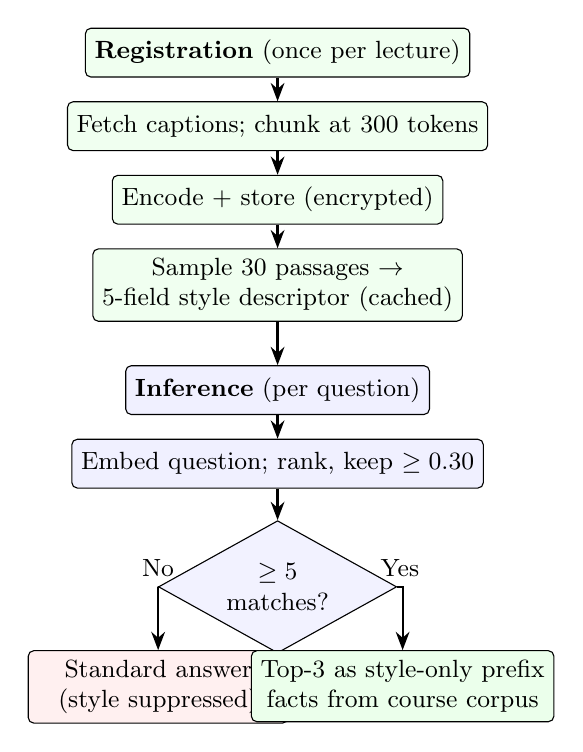
\begin{tikzpicture}[node distance=0.30cm]
\node[stage] (reg) {\textbf{Registration} (once per lecture)};
\node[stage, below=of reg] (chunk) {Fetch captions; chunk at 300 tokens};
\node[stage, below=of chunk] (embed) {Encode + store (encrypted)};
\node[stage, below=of embed] (fp) {Sample 30 passages $\to$\\5-field style descriptor (cached)};
\node[stage, below=0.55cm of fp, fill=blue!6] (inf) {\textbf{Inference} (per question)};
\node[stage, below=of inf, fill=blue!6] (rank) {Embed question; rank, keep $\geq 0.30$};
\node[dec, below=0.40cm of rank] (gate) {$\geq 5$\\matches?};
\node[stage, below left=0.38cm and -0.9cm of gate, fill=red!6] (fallback)
      {Standard answer\\(style suppressed)};
\node[stage, below right=0.38cm and -1.1cm of gate, fill=green!8] (apply)
      {Top-3 as style-only prefix\\facts from course corpus};
\draw[arr] (reg)--(chunk); \draw[arr] (chunk)--(embed);
\draw[arr] (embed)--(fp); \draw[arr] (fp)--(inf);
\draw[arr] (inf)--(rank); \draw[arr] (rank)--(gate);
\draw[arr] (gate) -| node[near start,above,font=\small]{No} (fallback);
\draw[arr] (gate) -| node[near start,above,font=\small]{Yes} (apply);
\end{tikzpicture}%
}
\caption{Persona engine: ingestion, fingerprinting, retrieval and gated
generation. Styling is suppressed unless five transcript passages clear the
relevance floor.}
\label{fig:persona}
\end{figure}

%------------------------------------------------
\section{Benchmark}
%------------------------------------------------
We constructed a curriculum QA benchmark of $174$ items: $150$ questions taken
verbatim from Karnataka Pre-University board papers across four subjects and
both years ($20$ per cell, except mathematics at $15$ where symbol-heavy
extraction reduced the yield), and $24$ authored degree-level questions outside
the syllabus that must be refused. Nothing in the answerable split is synthetic.
Gold answers are deliberately left for subject-teacher annotation: a benchmark
whose reference answers were written by the model family under evaluation would
be worthless. We therefore report abstention, retrieval economy, citation
behaviour and latency, and not answer correctness.

%------------------------------------------------
\section{Evaluation}
%------------------------------------------------
\subsection{Throughput and Retrieval Cost}
On the development host --- a $4$-core AMD Ryzen~5 7235HS, $11.7$\,GiB RAM, RTX
3050 with $4.0$\,GiB VRAM --- Qwen2.5-7B decodes at $4.7$ tokens/s on CPU and
$6.5$ at a $62/38$ CPU/GPU split, while Qwen2.5-3B reaches $19.6$ at $79\%$ GPU;
a 4-bit $7$B model needs $\approx 4.7$\,GiB and cannot be resident in $4.0$\,GiB.
Two consequences follow. The sub-five-second target is attainable only for short
tutoring answers, not practice-paper generation. And model choice is a
\emph{capability} decision: the $3$B model is four times faster but could not
emit a blueprint-conforming paper at all. Retrieval is negligible --- a median
$30$\,ms over forty questions ($18$\,ms encode, $2$\,ms dense search over all
$7{,}669$ passages, $9$\,ms BM25), $95$th percentile $54$\,ms --- under half a
percent of the $13$--$15$\,s end-to-end figures of Table~\ref{tab:ablation}.
Latency \emph{is} generation here.

\subsection{Exact-Term Recall}
Relevance is not annotated, so we measure the narrow property a lexical arm
should repair: for each of the $150$ answerable questions we take its rarest
content word by document frequency and ask at what rank the first passage
containing it appears in the top five. Dense retrieval alone reaches it for $91$
of $150$ at $\mathrm{MRR} = 0.493$; with the lexical arm fused in, $100$ of
$150$ at $0.566$, better on $32$ questions, worse on $3$. Two cautions: this is
exact-term recall, not relevance, so the gain is not an answer-quality gain; and
on fourteen hand-chosen queries the configurations were indistinguishable, an
artefact of a sample we chose ourselves.

\subsection{Ablation and the Evidence Floor}
\label{sec:ablation}
Table~\ref{tab:ablation} reports $48$ items per configuration ($40$ answerable,
$8$ out-of-syllabus). \textit{Scope note.} The items are the first in benchmark
order rather than a stratified sample, so all $40$ answerable items are
\emph{physics}; the ablation characterises one subject, and a stratified re-run
is the obvious next step.

\begin{table}[htbp]
\caption{Corrective-layer ablation (upper block) and evidence floor (lower
block), $48$ items per configuration from the physics split. \emph{Src.} is the
mean cited source references per response; \emph{P} and \emph{R} are abstention
precision and recall; \emph{Rest.} is passages restored past the grader. The
lower block is a paired re-run of the shipped configuration rather than the
published numbers, because generation is sampled.}
\label{tab:ablation}
\centering
\footnotesize
\setlength{\tabcolsep}{3.5pt}
\begin{tabular}{@{}lrrrrrr@{}}
\toprule
\textbf{Configuration} & \textbf{Src.} & \textbf{P} & \textbf{R} & \textbf{False} & \textbf{Rest.} & \textbf{Lat.\,(s)} \\
\midrule
Vanilla RAG              & 4.90 & \textbf{1.00} & 0.62 & \textbf{0} & --- & 13.3 \\
+ boilerplate filter     & 4.81 & \textbf{1.00} & 0.62 & \textbf{0} & --- & 14.0 \\
+ CRAG ($3$B grader)     & 1.08 & 0.42 & \textbf{1.00} & 11 & --- & \textbf{11.5} \\
+ filter + CRAG ($3$B)   & 1.08 & 0.53 & \textbf{1.00} & 7  & --- & 11.8 \\
+ filter + CRAG (strong) & 4.46 & 0.83 & 0.62 & 1  & --- & 17.1 \\
\midrule
filter\,+\,CRAG ($3$B)   & 1.02 & 0.47 & 0.88 & 8 & 0.00 & 13.1 \\
\quad +\,evidence floor  & 2.56 & 0.78 & 0.88 & 2 & 1.33 & 14.7 \\
\bottomrule
\end{tabular}
\end{table}

The result does not support this corrective configuration. With a $3$B grader
the layer refuses eleven of forty answerable questions, rejecting all five
retrieved passages for questions plainly in syllabus; recall reaches $1.00$ only
because the system has become indiscriminately reluctant, while precision
collapses from $1.00$ to $0.42$. Replacing only the grader isolates the cause:
sources recover to $4.46$ and false abstentions fall from seven to one, so the
failure lies in grader capacity, not the loop. The corrected system still does
not beat the plain baseline --- recall returns to $0.62$ while latency rises
$29\%$ --- and the boilerplate filter matches vanilla retrieval on every
abstention measure. An LLM-graded loop is bounded by its grader and below some
threshold is actively harmful.

Is that harm intrinsic, or is it the \emph{starvation} harsh grading produces?
The lower block answers it. Adding the evidence floor to the same $3$B grader
% Each CI endpoint closes its own math group so the double hyphen is an en-dash.
cuts false abstentions from eight to two of forty ($8/40$, 95\% Wilson CI:
$0.10$--$0.35$; $2/40$, 95\% Wilson CI: $0.01$--$0.17$), lifts abstention
precision from $7/15$ ($0.47$, 95\% Wilson CI: $0.25$--$0.70$) to $7/9$ ($0.78$,
95\% Wilson CI: $0.45$--$0.94$) and sources from $1.02$ to $2.56$, while
abstention recall is unchanged at $0.88$. Against the strong grader, which costs
a second model, the floor reaches comparable precision ($0.78$ against $0.83$)
with \emph{better} recall ($0.88$ against $0.62$) and lower latency ($14.7$
against $17.1$\,s). The harm is a starved generator rather than mistaken
ranking, and it is repairable without a stronger judge.

\subsection{Generator Capacity and Grounding}
\label{sec:faithfulness}
Holding retrieval fixed, we compared a local $3$B model against a stronger model
on identical passages. Asked to derive $F = ma$, the local model produced
Snell's law of refraction --- correct physics, but \emph{absent from the
retrieved context}; the stronger model stated that the derivation was not
present and declined. Retrieval gating and abstention are enforced in code and
hold regardless of model; everything downstream of ``the model is now
generating'' is advisory, and a small model does not reliably obey it.

The audit puts a number on this. Over the same $48$ items the shipped
configuration answered $37$ of $40$ answerable questions, and the audit read
back $8.1$ claims per answer, roughly $300$ checkable statements. A mean $0.781$
of an answer's claims are traceable to the retrieved passages, but only $0.065$
cite the passage carrying them: the model mostly writes from the material it was
given and almost never says which part. Twenty-eight of the $37$ answers
($76\%$) contain at least one untraceable statement. No answer cited a passage
never retrieved, a consequence of the low citation rate rather than a success.
The audit costs $14.5$\,s against $14.7$\,s without it, inside run-to-run
variation. Its \emph{accuracy}, as distinct from its cost, is unvalidated.

\subsection{Judged Quality and Persona Consistency}
\label{sec:judged}
Twenty-two answered items were scored twice over \emph{identical} answers, by
Qwen2.5-7B --- the generator's own family --- and by Gemini 2.5 Flash.
Faithfulness follows the RAGAS definition; relevancy is a direct judge rating,
not RAGAS's question-regeneration procedure. Across $n=22$ matched answers the
faithfulness scores correlate at $r = -0.074$ (95\% Fisher-$z$ CI: $-0.48$ to
$0.36$) --- a weak and imprecisely estimated association --- with mean absolute
difference $0.288$; faithfulness reads $0.676$ against $0.537$ and relevancy
$0.784$ against $0.832$. Much of the gap is mechanical: Gemini decomposes an
answer into $8.1$ statements where Qwen finds $4.3$. The rest is judgement; on
binary PSC labels agreement is $\kappa = 0.182$. Family separation did not
stabilise measurement, so we report the pair and the spread rather than a
headline value, and argue that lexical auditing and abstention --- needing no
judge --- deserve more weight.

The proposed PSC target was $0.78$ but was never pilot-calibrated. The judge
sees a persona-conditioned answer, three genuine excerpts from the registered
educator and three neutral passages, and labels it style-consistent. Twelve
questions were used; the persona engaged on $n=9$ and was suppressed on three
for want of five matching transcript passages. PSC among these $n=9$ activated
examples is $0.222$ by the same-family judge and $0.333$ by the cross-family
one, both far below $0.78$: the target is not met. Conditioning left lexical
grounding essentially unchanged ($0.943 \rightarrow 0.962$) and lengthened
answers by about $11\%$ --- close to quality-neutral.

The limitation is the encoder. A Hindi-caption lecture ($219{,}041$ embedding
tokens, truncated to $89{,}991$, yielding $360$ passages) produced a correct
style descriptor identifying Hindi--English code-switching, yet conditioning
never fired: an English question matches fewer than five Hindi passages, while a
Hindi question fails the course-evidence gate. The two requirements are mutually
exclusive under a monolingual encoder, and the five-passage floor correctly
suppressed styling rather than faking it. An English-caption lecture ($8{,}444$
tokens, $34$ passages) applied persona on the first attempt, with every numbered
citation resolving to the institutional textbook.

\subsection{System Output}
Fig.~\ref{fig:r-ask} shows a grounded answer with inline citation markers and a
\emph{Retrieved sources} list naming textbook file and page.
Fig.~\ref{fig:r-persona} shows the style descriptor with its passage count and
timestamped source links. Fig.~\ref{fig:r-grounding} makes the audit visible:
fourteen of sixteen statements trace to the retrieved passages, but \emph{none} carries
a citation identifying which.

\begin{figure}[!t]
\centering
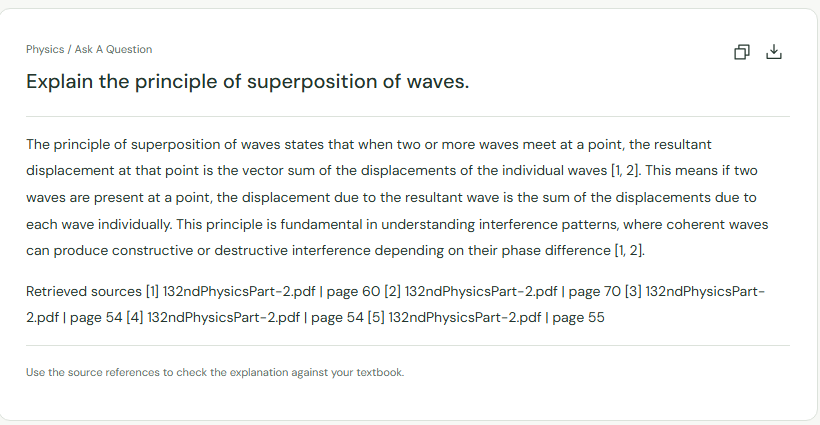
\includegraphics[width=\columnwidth]{figures/r01-ask-crop.png}
\caption{Grounded answer with inline citations resolving to textbook file and
page numbers.}
\label{fig:r-ask}
\end{figure}

\begin{figure}[!t]
\centering
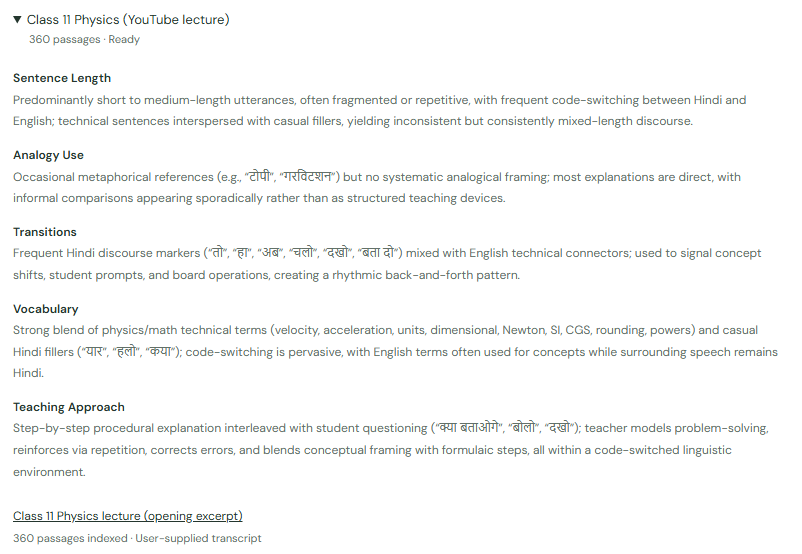
\includegraphics[width=\columnwidth]{figures/r07-persona-crop.png}
\caption{Style descriptor distilled from a registered educator's transcript,
with passage count and timestamped source attribution.}
\label{fig:r-persona}
\end{figure}

\begin{figure}[!t]
\centering
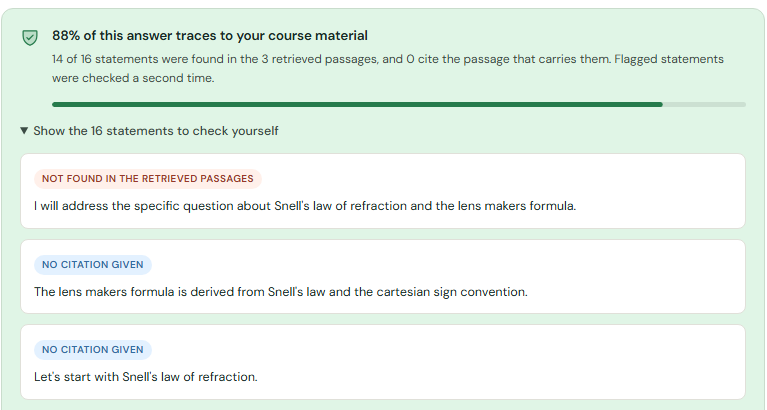
\includegraphics[width=\columnwidth]{figures/r09-grounding-crop.png}
\caption{The grounding audit beside an answer. Fourteen of sixteen statements are traceable to the retrieved passages while none cites the passage that supports
it, so the two shares are reported separately.}
\label{fig:r-grounding}
\end{figure}

%------------------------------------------------
\section{What Remains Unmeasured}
\label{sec:limits}
%------------------------------------------------
Several quantities have been measured; the remainder are open rather than
estimated. \textbf{Measurement validity.} PSC is measured but its judges
disagree ($\kappa = 0.182$), so the direction is dependable and the value is
not; settling it needs human raters and more than twelve questions. LLM-as-judge
circularity is measured and the news is bad: family separation was our proposed
mitigation, and the judges still fail to agree on identical answers; missing are
a human-rated calibration subset, position-swap debiasing and a larger panel.
The grounding audit is itself unvalidated --- we report how often it flags a
claim, not whether it is right to, and neither false-alarm nor miss rate is
known. \textbf{No human evaluation.} Judged faithfulness measures whether an
answer follows from the retrieved passages, not whether it is correct or would
earn marks; faculty annotation is incomplete, so we report no accuracy figure.
The TAM instrument~\cite{davis1989} and the $N \geq 30$ cohort were planned, not
executed. \textbf{Components described but not evaluated.} PYQ topic matching is
lexical, ranks single-token TF-IDF keywords, does not match differently worded
questions, and includes PDF artefacts, with no accuracy verified against a
teacher-labelled key. Practice papers are validated structurally, not
academically: board standard, Bloom-level fit and learning-outcome alignment are
content judgements needing faculty annotation. Speech coverage is declared, not
measured --- eight languages are accepted (English, Hindi, Kannada, Tamil,
Telugu, Malayalam, Marathi, Bengali) with Whisper (base) and synthesis disabled
by default, but we have measured word error rate for none, nor the downstream
effect of a transcription error. Diagram generation is likewise described, not
evaluated: re-emission makes output parseable by construction, a property of the
code rather than a measured result.

%------------------------------------------------
\section{Reproducibility}
\label{sec:repro}
%------------------------------------------------
The benchmark identifiers, ablation drivers and table-generation scripts are
available in the public artifact repository
(\url{https://github.com/Monish-Venkat/study-mate}). Board-paper questions and
textbook passages may be subject to third-party copyright: the distributable
artifact includes source identifiers, retrieval and annotation metadata and
reproduction scripts rather than redistributing protected passages without
permission. Each ablation restarts the service in every configuration it reports
and writes both Markdown and \LaTeX{}, so Table~\ref{tab:ablation} can be
regenerated rather than taken on trust, and the judged evaluation caches every
answer with the passages that produced it so a third judge can re-score
identical answers.

%------------------------------------------------
\section{Conclusion and Future Work}
%------------------------------------------------
We presented StudyMate and measured it rather than projecting it. Retrieval
already filtered by subject, level and board is hard to improve with a
corrective loop: a weak grader is actively harmful, a strong one costs latency
without measurably improving grounding, and a near-zero-cost boilerplate filter
matched both. The harm proved specific and cheap to fix --- a similarity-gated
evidence floor recovers most of what a strong grader buys without running one.
Grounding is better verified than instructed: across $300$ audited statements,
$78\%$ were traceable while only $6.5\%$ named the supporting passage. Persona
conditioning works with correct provenance separation, but only when the encoder
spans the languages involved. Two judges scoring identical answers do not agree,
so a reported LLM-judged faithfulness figure should name its judge with equal
prominence. Three lines of work follow: a multilingual encoder to restore
cross-lingual persona conditioning; teacher annotation to convert
board-conditioned generation into a measured claim scored blind by practising
examiners; and first-class treatment of abstention, which trades against
coverage in ways a single accuracy number hides. Federated corpus
sharing~\cite{fajardo2025} would let colleges pool material without centralising
student data.

%------------------------------------------------
\section*{Acknowledgment}
A plagiarism and AI-content similarity report generated with the
conference-recommended tool accompanies this manuscript as supplementary
material. The prose has been authored and revised by the student team.

%------------------------------------------------
\footnotesize
\begin{thebibliography}{26}
\bibitem{lewis2020}
P. Lewis et al., ``Retrieval-Augmented Generation for Knowledge-Intensive
NLP Tasks,'' \textit{Adv. Neural Inf. Process. Syst.}, vol. 33,
pp. 9459--9474, 2020.
\bibitem{bloom1984}
B. S. Bloom, ``The 2 Sigma Problem: The Search for Methods of Group
Instruction as Effective as One-to-One Tutoring,'' \textit{Educ.
Researcher}, vol. 13, no. 6, pp. 4--16, 1984.
\bibitem{vanlehn2011}
K. VanLehn, ``The Relative Effectiveness of Human Tutoring, Intelligent
Tutoring Systems, and Other Tutoring Systems,'' \textit{Educational
Psychologist}, vol. 46, no. 4, pp. 197--221, 2011.
\bibitem{lauber2025}
A.-M. Lauber, S. Martin, and B. Pampel, ``How Can I Help You? Didactic
Alignment for RAG Chatbots in Education,'' in \textit{Proc. 17th Int.
Conf. Educ. Technol. Comput. (ICETC)}, 2025, pp. 153--158.
\bibitem{teixeira2025}
S. Teixeira, M. Sonkaya, and P. Georgieva, ``RAG Augmented Large
Language Models as a Tool for Education,'' in \textit{Proc. Int. Conf.
Autom. Informatics (ICAI)}, 2025, pp. 769--774.
\bibitem{neumann2025}
A. T. Neumann, Y. Yin, S. Sowe, S. Decker, and M. Jarke,
``An LLM-Driven Chatbot in Higher Education for Databases and
Information Systems,'' \textit{IEEE Trans. Educ.}, vol. 68, no. 1,
pp. 103--112, 2025.
\bibitem{dong2025}
C. Dong, Y. Yuan, K. Chen, S. Cheng, and C. Wen, ``How to Build an
Adaptive AI Tutor for Any Course Using Knowledge Graph-Enhanced
Retrieval-Augmented Generation (KG-RAG),''
in \textit{Proc. 14th Int. Conf. Educational and Information Technology
(ICEIT)}, 2025, doi: 10.1109/ICEIT64364.2025.10975937.
\bibitem{nguyen2025}
L. Nguyen and T. Quan, ``URAG: Implementing a Unified Hybrid RAG for
Precise Answers in University Admission Chatbots,''
\textit{arXiv preprint arXiv:2501.16276}, 2025.
\bibitem{zhao2024}
Z. Zhao, Z. Yin, J. Sun, and P. Hui, ``Embodied AI-Guided Interactive
Digital Teachers for Education,'' in \textit{SIGGRAPH Asia Educators
Forum}, ACM, 2024.
\bibitem{he2025}
S. He, L. Liu, J. Ma, and Y. Lu, ``RAG-X-Driven Construction of an
Intelligent Platform for Teaching Assistance in Higher Education,''
in \textit{Proc. 5th Int. Conf. Educ. Technol. (ICET)}, 2025,
pp. 238--242.
\bibitem{luo2026}
Y. Luo, D. R. Sarkar, R. H. Sangree, and S. Goswami,
``ARIA: Adaptive Retrieval Intelligence Assistant---A Multimodal RAG
Framework for Domain-Specific Engineering Education,''
\textit{arXiv preprint arXiv:2604.06179}, 2026.
\bibitem{koutsiaki2025}
M. E. Koutsiaki et al., ``From Textbook to Talkbot: A Case Study of a
Greek-Language RAG-Based Chatbot in Higher Education,'' in
\textit{Proc. Barcelona Conf. Educ.}, 2025.
\bibitem{gielis2025}
F. L\'opez-Ostenero, J. Mart\'inez-Romo, L. Plaza, and L. Araujo,
``Personalized Self-Assessment Tool Using a Telegram Bot: A Case Study on
Data Structures and Algorithms,'' in \textit{Proc. IEEE Global Engineering
Education Conf. (EDUCON)}, 2024, pp. 1--8,
doi: 10.1109/EDUCON60312.2024.10578697.
\bibitem{es2025}
S. Es, J. James, L. Espinosa-Anke, and S. Schockaert,
``RAGAS: Automated Evaluation of Retrieval Augmented Generation,''
in \textit{Proc. 18th Conf. Eur. Chapter Assoc. Comput. Linguistics: System
Demonstrations}, pp. 150--158, 2024, doi: 10.18653/v1/2024.eacl-demo.16.
\bibitem{davis1989}
F. D. Davis, ``Perceived Usefulness, Perceived Ease of Use, and User
Acceptance of Information Technology,'' \textit{MIS Quart.}, vol. 13,
no. 3, pp. 319--340, 1989.
\bibitem{roh2021}
Y. Roh, G. Heo, and S. E. Whang, ``A Survey on Data Collection for
Machine Learning: A Big Data--AI Integration Perspective,''
\textit{IEEE Trans. Knowl. Data Eng.}, vol. 33, no. 4,
pp. 1328--1347, 2021.
\bibitem{kuhail2023}
M. A. Kuhail et al., ``Interacting with Educational Chatbots: A
Systematic Review,'' \textit{Educ. Inf. Technol.}, vol. 28, no. 1,
pp. 973--1018, 2023.
\bibitem{wollny2021}
A. Wollny et al., ``Are We There Yet? A Systematic Literature Review on
Chatbots in Education,'' \textit{Front. Artif. Intell.}, vol. 4,
p. 654924, 2021.
\bibitem{fajardo2025}
V. A. Fajardo et al., ``FedRAG: A Framework for Fine-Tuning
Retrieval-Augmented Generation Systems,''
\textit{arXiv preprint arXiv:2506.09200}, 2025.
\bibitem{yan2024crag}
S.-Q. Yan, J.-C. Gu, Y. Zhu, and Z.-H. Ling, ``Corrective Retrieval
Augmented Generation,'' \textit{arXiv preprint arXiv:2401.15884}, 2024.
\bibitem{robertson2009}
S. Robertson and H. Zaragoza, ``The Probabilistic Relevance Framework: BM25
and Beyond,'' \textit{Foundations and Trends in Information Retrieval},
vol. 3, no. 4, pp. 333--389, 2009.
\bibitem{cormack2009}
G. V. Cormack, C. L. A. Clarke, and S. B\"{u}ttcher, ``Reciprocal Rank Fusion
Outperforms Condorcet and Individual Rank Learning Methods,'' in
\textit{Proc. 32nd ACM SIGIR}, 2009, pp. 758--759.
\bibitem{manakul2023}
P. Manakul, A. Liusie, and M. J. F. Gales, ``SelfCheckGPT: Zero-Resource
Black-Box Hallucination Detection for Generative Large Language Models,'' in
\textit{Proc. EMNLP}, 2023, pp. 9004--9017.
\bibitem{gao2023}
T. Gao, H. Yen, J. Yu, and D. Chen, ``Enabling Large Language Models to
Generate Text with Citations,'' in \textit{Proc. EMNLP}, 2023,
pp. 6465--6488.
\bibitem{liu2024persona}
Z. Liu, S. X. Yin, G. Lin, and N. F. Chen, ``Personality-Aware Student
Simulation for Conversational Intelligent Tutoring Systems,'' in
\textit{Proc. EMNLP}, 2024, pp. 626--642.
\bibitem{liu2025pace}
H. Liu, Z. Zhang, G. Lin, Y. Jia, and H. Peng, ``One Size Doesn't Fit All: A
Personalized Conversational Tutoring Agent for Mathematics Instruction,''
\textit{arXiv preprint arXiv:2502.12633}, 2025.
\end{thebibliography}
\end{document}
